\documentclass[letterpaper]{article}
\usepackage[submission]{aaai2027}
\usepackage[hyphens]{url}
\usepackage{graphicx}
\urlstyle{rm}
\def\UrlFont{\rm}
\usepackage{natbib}
\usepackage{caption}
\frenchspacing
\usepackage{algorithm}
\usepackage{algorithmic}
\usepackage{booktabs}
\usepackage{amsmath,amssymb,amsthm}
\pdfinfo{/TemplateVersion (2027.1)}
\setcounter{secnumdepth}{2}

\theoremstyle{plain}
\newtheorem{proposition}{Proposition}
\newcommand{\X}{\mathcal{X}}
\newcommand{\D}{\mathcal{D}}

\title{Supplementary Material:\\Decomposing the GP Advantage in Offline MBO}
\author{Anonymous Submission}
\affiliations{}

\begin{document}
\maketitle

This supplement contains the proofs of Propositions~1--2, the full per-method result tables, the identifiability (matched-tuning) control, the $\beta$ and ensemble-size ablations, the official-baseline cross-check, the significance details, and the complete experimental configuration. It is provided for reproducibility and is not part of the 7-page body.

\section{Proofs}

\paragraph{Notation.} Objective $f:\X\to\mathbb{R}$; surrogate posterior mean $\mu$ and uncertainty $\sigma>0$; LCB $L_\beta(x)=\mu(x)-\beta\sigma(x)$, $\beta\ge0$. For a distribution $Q$ on $\X$, $L_\beta$ is a \emph{valid $(1{-}\delta)$ lower bound under $Q$} if $\Pr_{x\sim Q}(f(x)\ge L_\beta(x))\ge 1{-}\delta$.

\begin{proposition}[Coverage of the premise is LCB validity]
For any $Q,\beta,\delta$,
$\Pr_{x\sim Q}(f(x)\ge L_\beta(x))=\Pr_{x\sim Q}(\mu(x)-f(x)\le\beta\sigma(x))$,
so $L_\beta$ is a valid $(1{-}\delta)$ lower bound under $Q$ iff the premise $\{\mu-f\le\beta\sigma\}$ has $Q$-probability at least $1{-}\delta$.
\end{proposition}
\begin{proof}
Since $\sigma>0$, pointwise $f(x)\ge\mu(x)-\beta\sigma(x)\iff\mu(x)-f(x)\le\beta\sigma(x)$. The two events coincide as subsets of $\X$ and hence have equal probability under any $Q$.
\end{proof}
\noindent\emph{Sanity checks.} $\beta{=}0$ gives $\Pr(f\ge\mu)=\Pr(\mu-f\le0)$; $\beta\to\infty$ gives coverage $\to1$. The identity is dimensionless and uses $\sigma>0$ once.

\begin{proposition}[Split-conformal repair; shift-limited transfer]
Let $\{(x_i,f(x_i))\}_{i=1}^n$ be exchangeable from $P$, $r_i=(\mu(x_i)-f(x_i))/\sigma(x_i)$ the signed one-sided nonconformity, and $\hat q$ the $\lceil(n{+}1)(1{-}\delta)\rceil$-th smallest of $r_1,\dots,r_n$. Then for a fresh $x_{n+1}\sim P$ exchangeable with the calibration set,
$\Pr(f(x_{n+1})\ge\mu(x_{n+1})-\hat q\,\sigma(x_{n+1}))\ge 1{-}\delta$.
Under a shifted proposal $\Pi\neq P$ with density ratio $w=d\Pi/dP$, validity is restored by weighting the calibration quantile by $w$ (weighted conformal).
\end{proposition}
\begin{proof}
The normalized scores $r_1,\dots,r_{n+1}$ are exchangeable, so by the split-conformal rank argument $\Pr(r_{n+1}\le\hat q)\ge1{-}\delta$. The event $r_{n+1}\le\hat q$ implies $\mu(x_{n+1})-f(x_{n+1})\le\hat q\,\sigma(x_{n+1})$, i.e.\ $f(x_{n+1})\ge\mu-\hat q\sigma$; monotonicity of probability gives the bound. The covariate-shift clause is the weighted-exchangeability extension of \citet{tibshirani2019conformal}: replacing the empirical quantile of $\{r_i\}$ with its $w$-weighted analogue restores marginal validity under $\Pi$. At $\Pi=P$, $w\equiv1$ recovers the unweighted bound.
\end{proof}

\paragraph{The shift clause is stated for completeness and is not applied.} The weighted extension requires a \emph{known} density ratio $w$, and that is the form in which the guarantee holds; the estimated case is supported empirically rather than by a theorem bounding the coverage gap \citep{tibshirani2019conformal}, and weighted procedures are exact when the magnitude of the shift is known \citep{angelopoulos2023conformal}. Here $\Pi$ is the distribution of designs an optimizer proposes after ascending a surrogate---the setting in which $w$ is least knowable, and arguably not well defined, since the proposals are the deterministic output of an optimization concentrated on a low-dimensional set. We neither estimate $w$ nor apply weighted conformal anywhere in this paper. The clause is recorded because the proposition would be incomplete without it, not because it is available to us.

That unavailability is itself the explanation for a result reported below. Table~\ref{tab:cov} shows split-conformal repair restoring in-distribution coverage to its $0.90$ target on \emph{every} task while leaving out-of-distribution coverage erratic---spanning $0.00$ to $1.00$ there, with exactly $0.00$ on four of the fourteen tasks. That contrast is engine-robust, which is why we rest on it: recomputed on the audited engine the same repair again hits $0.90$ on all seven synthetic tasks while OOD coverage again scatters, from $0.11$ to $1.00$. The floor differs between engines; the pattern does not. Unweighted split conformal is valid under exchangeability, which the optimizer's proposals violate by construction, and the weighting that would repair the shift needs the $w$ we have just said is unavailable. So the erratic OOD column is what the theory predicts rather than an anomaly, and it reinforces the separate finding that premise coverage is separable from optimization outcome: a procedure can be made to cover in-distribution without that touching where the optimizer actually goes.

\section{Full Result Tables}

Table~\ref{tab:sfull} reports the full synthetic grid including the domain baselines (COMs, CbAS, gradient ascent); Table~\ref{tab:srank} the corresponding average ranks. The ensemble$\times$gradient and gradient-ascent/COMs rows are the boundary-collapse cells discussed in the body. Both tables are on the \emph{uncorrected} engine, which is stated in each caption and mapped in Section~\ref{sec:enginemap}: they are the grid as previously published, retained so that the corrections in the body can be read against what they corrected. Every number the body asserts is on the audited engine instead.

\begin{table*}[t]\centering
\caption{Full synthetic grid, 100th-percentile score (30 seeds), including domain baselines, on the \emph{uncorrected} engine---X1 off and X3 off, i.e.\ the ensemble trains on raw targets and the candidate/oracle protocol is unequalized. \textbf{Bold} = best per task. The body reports the audited corner (X1 and X3 on) throughout, so cell values here are not the body's; Section~\ref{sec:enginemap} maps every supplementary number to its engine.}
\label{tab:sfull}
\setlength{\tabcolsep}{5pt}\small
\begin{tabular}{lccccccc}
\toprule
Method & Branin & Styblinski & Levy & Rosenbrock & Rastrigin & Ackley & Griewank \\
\midrule
Ens+Grad & $-9.27$ & $6.34$ & $-2.14$ & $-0.28$ & $-7.71$ & $-3.66$ & $-2592$ \\
Ens+Pert & $-0.78$ & $33.03$ & $-0.40$ & $-0.12$ & $-8.44$ & $-6.32$ & $-395$ \\
Ens+CMA & $-14.01$ & $5.15$ & $-3.19$ & $-0.48$ & $-10.81$ & $-4.31$ & $-2613$ \\
GP+Grad & $\mathbf{-0.40}$ & $27.57$ & $\mathbf{-0.05}$ & $-0.09$ & $-4.83$ & $\mathbf{-0.55}$ & $\mathbf{-0.94}$ \\
GP+Pert & $-0.40$ & $\mathbf{36.15}$ & $-0.24$ & $-0.08$ & $-8.28$ & $-6.28$ & $-270$ \\
GP+CMA & $-0.40$ & $26.65$ & $-0.05$ & $-0.09$ & $-5.06$ & $-0.59$ & $-1.00$ \\
SVGP+Grad & $-0.45$ & $11.83$ & $-0.08$ & $\mathbf{-0.04}$ & $\mathbf{-2.83}$ & $-0.70$ & $-2.09$ \\
SVGP+Pert & $-0.40$ & $34.31$ & $-0.25$ & $-0.08$ & $-8.27$ & $-6.14$ & $-275$ \\
SVGP+CMA & $-0.53$ & $11.53$ & $-0.08$ & $-0.04$ & $-2.99$ & $-0.74$ & $-2.15$ \\
COMs & $-9.73$ & $8.21$ & $-4.44$ & $-1.31$ & $-6.97$ & $-4.49$ & $-2078$ \\
CbAS & $-5.64$ & $33.85$ & $-0.21$ & $-0.05$ & $-8.02$ & $-5.10$ & $-276$ \\
Grad.\ Asc. & $-8.35$ & $3.51$ & $-2.43$ & $-0.31$ & $-9.08$ & $-3.04$ & $-2701$ \\
\bottomrule
\end{tabular}
\end{table*}

\begin{table}[t]\centering
\caption{Average rank over the 7 synthetic tasks (derived from Table~\ref{tab:sfull}, so likewise the \emph{uncorrected} X1-off/X3-off engine; lower is better).}
\label{tab:srank}
\small
\begin{tabular}{lc@{\hskip 2em}lc}
\toprule
Method & Rank & Method & Rank \\
\midrule
GP+Grad   & $2.57$ & GP+Pert    & $5.71$ \\
SVGP+Grad & $3.29$ & SVGP+Pert  & $5.86$ \\
GP+CMA    & $3.57$ & CbAS       & $6.00$ \\
SVGP+CMA  & $4.29$ & Ens+Pert   & $8.14$ \\
Ens+Grad  & $8.57$ & COMs       & $9.43$ \\
Grad.Asc. & $9.86$ & Ens+CMA    & $10.71$ \\
\bottomrule
\end{tabular}
\end{table}

\section{Identifiability: Matched Tuning (GATE-1)}
Exact and sparse GPs can spend per-run marginal-likelihood budget that ensembles cannot. The \emph{matched} arm freezes GP hyperparameter fitting so every surrogate receives the same (zero) per-run tuning budget. The surrogate main effect on synthetic tasks is $\eta^2_{\text{surr}}{=}0.37$ unmatched and $0.28$ matched---a $75\%$ retention. Both figures are on the \emph{uncorrected} engine, matching Table~\ref{tab:sfull} rather than the body's audited corner; the control is a within-engine contrast, so what it licenses is the retention ratio and not either level. The optimizer main effect stays small in both ($\eta^2_{\text{opt}}{=}0.01\to0.02$) and the interaction stays large ($\eta^2_{\text{inter}}{=}0.17\to0.12$). The GP advantage is therefore a surrogate-class property, not a per-run tuning artifact.

\section{Mechanism Controls}
The Section-5 mechanism rests on three controls, all on the synthetic tasks (task-normalized, averaged over optimizers).

\paragraph{Pessimism off ($\beta{=}0$).} Re-running the full $3\times3$ grid at $\beta{=}0$ (no $\sigma$ penalty) and reading both conditions on a single $\beta$-invariant normalizer, the GP--ensemble marginal gap is $0.319$ $[0.196,0.460]$ at $\beta{=}0$ against $0.525$ $[0.406,0.614]$ at $\beta{=}2$. Two things follow, and both are asserted. First, $61\%$ of the advantage survives with $\sigma$ removed entirely and the interval excludes zero, so the advantage rests on a substantial mean-quality base. Second, the paired increment is $0.203$ $[0.007,0.396]$ with $p{=}0.020$, which \emph{excludes} zero: pessimism is a significant amplifier of that base, not a bystander. A normalization-free cross-check (per-task $z$-score by the task's own pooled cell-mean standard deviation) gives $0.904$ and $1.473$ standard deviations respectively---the same $0.61$ ratio---so the conclusion is not an artifact of min--max scaling. Per-task, the ensemble$\times$gradient cell still collapses without pessimism (Griewank $-42.7$, Rastrigin $-9.5$) while the GP does not (Griewank $-0.96$); these are the audited $\beta{=}0$ grid's own cell means, on the same engine as the interval above.

Two cautions on these numbers. The per-task gaps are heterogeneous: on Branin the $\beta{=}0$ gap ($0.664$) \emph{exceeds} its $\beta{=}2$ gap ($0.468$), while on Griewank-30D the $\beta{=}0$ gap is nearly absent ($0.098$); at $n{=}7$ this spread is descriptive only. And the figures above are \emph{not} comparable to gaps computed with a normalizer refit separately at each $\beta$, which express the two conditions in different units; such figures may be read within a $\beta$ condition but never as a cross-$\beta$ ratio.

\paragraph{Matched subsample.} Training the ensemble on the GP's score-biased $800$-point subsample rather than all data \emph{widens} the gap to $0.76$ (the ensemble marginal falls from $0.34$ to $0.08$): the GP wins with less data, so the biased subsample is not its edge. This control is computed on the legacy per-condition normalizer and is \emph{not} on the same ruler as the $\beta{=}0$ figures above; only its direction should be read across the two.

\paragraph{Cross-proposal coverage.} Table~\ref{tab:cross} measures each surrogate's premise coverage in-distribution, on its own proposals, and on the other surrogate's proposals. The ensemble premise holds in-distribution ($0.73$) and on the GP's proposals ($0.97$) but collapses on its own ($0.42$); the GP premise holds on both ($0.97$). The ensemble is not miscalibrated in general---only where its own gradient optimizer drives it.

That last sentence points the same way as the interaction reported in the body, and the two are worth reading together---though they are not the same measurement, and we state the difference rather than eliding it. Premise validity here is a property of a \emph{pair} rather than of the surrogate alone: the same ensemble premise holds at $0.97$ on points the GP's pipeline proposed and collapses to $0.42$ on points its own pipeline proposed. What varies across those two columns is the proposal source---a different surrogate, driven by its own optimizer---so this is a surrogate$\times$proposal-source contrast and not a direct read-out of the surrogate$\times$optimizer interaction the ANOVA estimates. It is corroborating evidence that premise validity is pair-dependent, not a second estimate of $\eta^2_{\text{inter}}$. Coverage figures are probabilities rather than min--max normalized scores, so the $0.42$-versus-$0.97$ contrast is untouched by the normalizer critique that bears on every $\eta^2$ in this paper. As stated in the body, the $0.97$ premise-coverage value belongs to the scikit-learn exact GP rather than the differentiable GP the grid scores; the repository carries both implementations.

\paragraph{Simple effects.} Once an interaction is significant, main effects can mislead, and the standard remedy for a $3\times3$ design is to report the simple effects alongside the two main effects. Table~\ref{tab:simple} gives $\eta^2_{\text{surr}}$ conditional on each optimizer, computed from the stored per-seed data on the \emph{shared omnibus normalizer}. That sharing matters and is easy to get wrong: re-normalizing within a single optimizer's three cells inflates the perturbation figure to roughly $0.73$, because min--max rescaling to any three points restores a full unit spread by construction. The perturbation column sits between $0.004$ and $0.020$ in every corner against $0.39$--$0.81$ for the two aggressive optimizers, so the asymmetry is corner-invariant in the same way the interaction is. The two X1-off corners retain the target-scaling confound, which is why their intervals are widest.

\begin{table}[t]\centering
\caption{Simple effects: $\eta^2_{\text{surr}}$ conditional on each optimizer, shared omnibus normalizer, all four engine corners. The primary corner is bold.}
\label{tab:simple}
\small
\begin{tabular}{lccc}
\toprule
Corner & at perturbation & at gradient & at CMA \\
\midrule
off / off & $0.004$ & $0.666$ & $0.814$ \\
on\ \,/ off & $0.004$ & $0.388$ & $0.763$ \\
off / on\ \, & $0.019$ & $0.790$ & $0.813$ \\
on\ \,/ on\ \, & $\mathbf{0.007}$ & $\mathbf{0.735}$ & $\mathbf{0.762}$ \\
\bottomrule
\end{tabular}
\end{table}

\paragraph{The same asymmetry in raw oracle units.} The simple-effects table is computed on normalized scores. The identical pattern is visible without any normalization at all, which is why we report both: Table~\ref{tab:rawgap} gives the gap between the better GP class and the ensemble in raw oracle units, per task and per optimizer, on the audited engine. The perturbation gap is smaller than both aggressive-optimizer gaps on all seven tasks. These are two views of one asymmetry rather than two independent findings---the raw-units form is the interaction expressed in units the normalizer critique cannot reach---and neither view establishes the causal reading, for the floor-effect reason given in the body.

\begin{table}[t]\centering
\caption{Exact-GP-minus-ensemble gap in raw oracle units (audited engine, X1 and X3 on, $\beta{=}2$, $K{=}5$, 30 seeds). ``GP'' is the exact GP throughout, matching the GP rows of Table~\ref{tab:sfull}; we use the single class rather than the better of the two per cell, since a per-cell maximum would be a selection statistic. Last column: perturbation gap as a percentage of the larger aggressive-optimizer gap. The negative entry on Ackley is the limiting case of the same pattern---there the ensemble edges the exact GP by $0.004$ under perturbation, so the gap has not merely shrunk but closed.}
\label{tab:rawgap}
\setlength{\tabcolsep}{4pt}\small
\begin{tabular}{lcccc}
\toprule
Task & gradient & perturbation & CMA & pert.\ \% \\
\midrule
Branin-2D      & $6.95$   & $0.053$  & $6.71$   & $0.8$ \\
Styblinski-5D  & $15.13$  & $5.996$  & $14.65$  & $39.6$ \\
Levy-8D        & $0.46$   & $0.047$  & $0.53$   & $8.8$ \\
Rosenbrock-10D & $0.09$   & $0.008$  & $0.10$   & $7.9$ \\
Rastrigin-15D  & $4.92$   & $0.187$  & $5.81$   & $3.2$ \\
Ackley-20D     & $5.10$   & $-0.004$ & $5.32$   & $-0.1$ \\
Griewank-30D   & $288.46$ & $25.556$ & $321.78$ & $7.9$ \\
\bottomrule
\end{tabular}
\end{table}

\paragraph{Small-$n$ bias in $\eta^2$.} $\eta^2$ is positively biased at small $n$, and we disclose the size of that bias from our own artifacts rather than citing it in the abstract. Across the four corners the bootstrap mean exceeds the point estimate by $+0.0160$, $+0.0184$, $+0.0123$ and $+0.0099$ for the surrogate effect, which is the direction and rough magnitude the simulation literature reports \citep{okada2013epsilon}. Bias-correcting gives $0.351$, $0.264$, $0.438$ and $0.395$ against the reported $0.367$, $0.283$, $0.450$ and $0.405$. The two-confound comparison therefore moves $0.351\to0.395$ under correction, an increment of $+0.0437$ against the $+0.0376$ of the uncorrected pair: the direction survives and the magnitude of the change grows slightly. The interaction survives correction at $0.156$, $0.134$, $0.147$ and $0.156$. We name $\epsilon^2$ rather than $\omega^2$ as the correction because the simulation evidence identifies $\epsilon^2$ as the least biased of the standard indices, against a common preference for $\omega^2$ \citep{okada2013epsilon}.

\paragraph{An independent reproduction of the headline scalar.} The $\beta$ sweep and the corner decomposition are separate runs that meet at one operating point: both sit at X1 and X3 on, $\beta{=}2$, $K{=}5$, 30 seeds. They are genuinely independent rather than the same numbers twice---their per-cell means differ on 58 of the 63 cells, since the two runs draw different random streams---and they nonetheless give $\eta^2_{\text{surr}}=0.40636$ from the $\beta$-sweep endpoint against $0.40455$ from the headline corner, landing $0.0018$ apart. For a scalar whose central challenge is that it is an operating-point artifact, an independent reproduction at the same operating point is worth stating explicitly rather than leaving a reader to read the two figures as one number rounded twice.

\begin{table}[t]\centering
\caption{Premise coverage at $\beta{=}2$ (synthetic mean), each surrogate on in-distribution points, its own proposals, and the other surrogate's proposals. Uncorrected engine (X1 off / X3 off), as in Table~\ref{tab:sfull}. ``Other's proposals'' means the points the \emph{other surrogate's} pipeline returned, so this table crosses surrogate against proposal source, not against optimizer.}
\label{tab:cross}
\small
\begin{tabular}{lccc}
\toprule
Premise & in-dist & own prop. & other's prop. \\
\midrule
Ensemble & $0.73$ & $0.42$ & $0.97$ \\
GP       & $0.98$ & $0.97$ & $0.93$ \\
\bottomrule
\end{tabular}
\end{table}

\section{Ablations}
\paragraph{Pessimism strength $\beta$.} Sweeping $\beta\in\{0,0.5,1,2,5\}$ (the $\beta$-resolution curve is Figure~3 of the main paper), increasing pessimism improves the final score on 6 of 7 synthetic tasks (median normalized slope $+0.19$); the exception is Ackley, where the uninformative $\sigma$ makes the penalty point away from the optimum. That the benefit is distance-regularization rather than calibrated conservatism is confirmed by Figure~\ref{fig:calib}: the per-task calibration quality $\rho$ (rank correlation between $\sigma$ and $|\mu-f|$) does not predict whether pessimism helps.
\paragraph{Ensemble size $K$.} $K$ is treated throughout as a confound to be controlled, never as a discovered mechanism. Sweeping $K\in\{2,3,5,10\}$ on the audited engine (Figure~\ref{fig:k}), two facts are reported with equal weight. \emph{Sensitivity:} $\eta^2_{\text{surr}}$ is $K$-dependent---$0.326$, $0.366$, $0.408$, $0.389$---peaking at exactly the $K{=}5$ the field fixes by convention, so the headline magnitude sits at the effect's maximum and we say so. \emph{Non-reversal:} the ranking does \emph{not} flip at $K{=}2$, where the ensemble marginal is $0.283$ against the GP's $0.767$. Our range $K\in\{2,3,5,10\}$ shares three of its four points with the $K\in\{2,5,10\}$ over which ensemble surrogates were reported robust in online BO under a fixed acquisition rule \citep{li2024bnnsurrogates}, adding only $K{=}3$; we claim no priority on the range, which already reached $K{=}2$. The residual is that the two sweeps measure different quantities: that work asks whether ensemble-BO \emph{performance} is robust to $K$ and finds that it is, while we ask whether the variance \emph{attributed to the surrogate axis} is robust to $K$ and find that it is not. Both can hold simultaneously, and only the second bears on a decomposition. Our pre-registered kill criterion for this sweep---that an ensemble marginal exceeding the GP's at $K{=}2$ would overturn the headline---did not fire.

The monotonically decreasing task-normalized score reported in an earlier draft of this supplement ($0.95$ at $K{=}2$) \emph{does not reproduce} on the audited engine, which gives $0.283$ at that cell. That figure is withdrawn, and no claim in this paper rests on it.

\begin{figure}[t]\centering
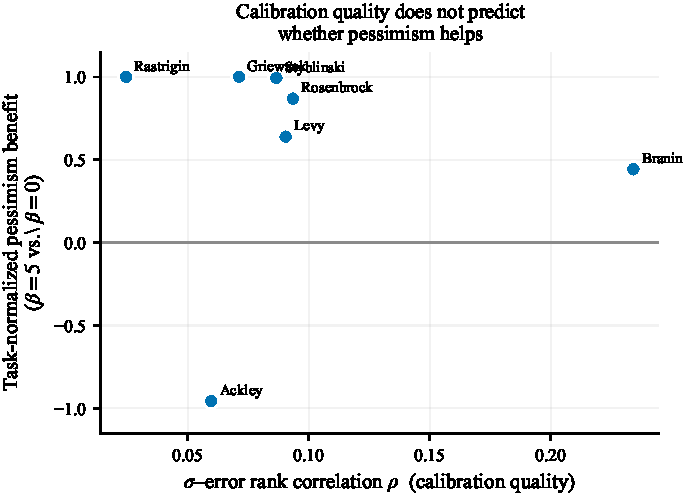
\includegraphics[width=0.9\columnwidth]{figures/fig5_calibration_vs_benefit}
\caption{Calibration quality vs.\ pessimism benefit. Each point is a synthetic task; the $\sigma$--error rank correlation $\rho$ (x-axis) does not predict the gain from pessimism (y-axis), consistent with a regularization rather than calibration effect.}
\label{fig:calib}
\end{figure}
\begin{figure}[t]\centering
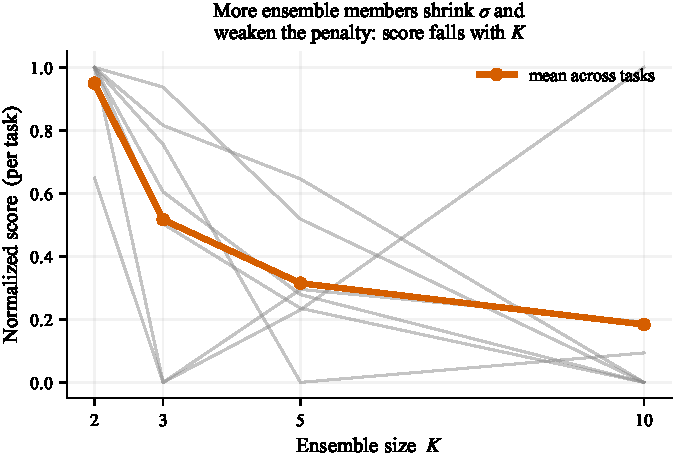
\includegraphics[width=0.9\columnwidth]{figures/fig7_k_ablation}
\caption{Ensemble-size ablation. Task-normalized score decreases with $K$.}
\label{fig:k}
\end{figure}

\section{Official-Baseline Cross-Check}
We ran the official \texttt{design-baselines} COMs and CbAS and compare to our reimplementations on the normalized scale (Table~\ref{tab:cc}). CbAS matches closely (TF-Bind-8 $|\Delta|{=}0.004$); COMs diverges (TF-Bind-8 $|\Delta|{=}1.22$), reflecting a reduced-epoch official run and a different oracle variant. We therefore report both rather than a single number.

\begin{table}[t]\centering
\caption{Official vs.\ reimplemented baselines (normalized 100th-percentile).}
\label{tab:cc}
\small
\begin{tabular}{llccc}
\toprule
Method & Task & Official & Ours & $|\Delta|$ \\
\midrule
COMs & Superconductor & $1.31$ & $1.01$ & $0.30$ \\
COMs & TF-Bind-8      & $0.99$ & $2.21$ & $1.22$ \\
COMs & GFP            & $-8.38$& $-9.20$& $0.82$ \\
CbAS & Superconductor & $1.21$ & $1.36$ & $0.15$ \\
CbAS & TF-Bind-8      & $2.13$ & $2.12$ & $\mathbf{0.004}$ \\
CbAS & GFP            & $2.20$ & $1.85$ & $0.35$ \\
\bottomrule
\end{tabular}
\end{table}

\section{Per-Task Premise Coverage}
Table~\ref{tab:cov} gives the per-task one-sided coverage of the pessimism premise at $\beta{=}2$, with the fitted split-conformal multiplier $\hat q$ and the repaired coverages. In-distribution coverage is moderate-to-high and on several real tasks above nominal (the ensemble under-predicts there, giving negative $\hat q$); OOD coverage is task-dependent, near zero exactly on the tasks where gradient ascent collapses. Conformal restores in-distribution coverage to its $0.90$ target on every task but leaves OOD coverage erratic. GFP is degenerate---coverage is measured on relaxed logits and is a decode artifact rather than a calibration signal.

\begin{table}[t]\centering
\caption{One-sided coverage of the premise $\mu{-}f\le\beta\sigma$ (i.e.\ $f\ge\mu-\beta\sigma$) at $\beta{=}2$ (nominal $0.90$). $c_{\text{in}}/c_{\text{ood}}$: coverage in-distribution / on proposals; $\hat q$: signed split-conformal multiplier (negative $\Rightarrow$ the mean already over-covers); $c^{\text{cf}}$: coverage after replacing $\beta$ with $\hat q$. Uncorrected engine (X1 off / X3 off), as in Table~\ref{tab:sfull}. On the audited engine the same measurement moves substantially---Branin's $c_{\text{in}}$ is $0.82$ rather than $0.71$ and its $c_{\text{ood}}$ $0.13$ rather than $0.35$---because the two corrections change what the optimizer proposes, which is exactly where OOD coverage is read. The qualitative pattern is the same on both engines and is the only thing we draw on: conformal repairs in-distribution coverage to $0.90$ on every task and leaves OOD coverage erratic.}
\label{tab:cov}
\setlength{\tabcolsep}{4pt}\small
\begin{tabular}{lccccc}
\toprule
Task & $c_{\text{in}}$ & $c_{\text{ood}}$ & $\hat q$ & $c^{\text{cf}}_{\text{in}}$ & $c^{\text{cf}}_{\text{ood}}$ \\
\midrule
Branin      & $0.71$ & $0.35$ & $6.6$  & $0.90$ & $0.77$ \\
Styblinski  & $0.66$ & $0.00$ & $7.2$  & $0.90$ & $0.02$ \\
Levy        & $0.68$ & $0.10$ & $6.0$  & $0.90$ & $0.40$ \\
Rosenbrock  & $0.86$ & $0.69$ & $2.5$  & $0.90$ & $0.71$ \\
Rastrigin   & $0.73$ & $0.79$ & $4.8$  & $0.90$ & $0.83$ \\
Ackley      & $0.92$ & $1.00$ & $1.9$  & $0.90$ & $1.00$ \\
Griewank    & $0.57$ & $0.00$ & $15.9$ & $0.90$ & $0.07$ \\
\midrule
TF-Bind-8      & $0.92$ & $0.71$ & $1.7$  & $0.90$ & $0.70$ \\
TF-Bind-10     & $1.00$ & $0.51$ & $-1.6$ & $0.89$ & $0.44$ \\
Superconductor & $1.00$ & $0.01$ & $-2.1$ & $0.90$ & $0.00$ \\
GFP            & $0.00$ & $0.00$ & $67.4$ & $0.90$ & $1.00$ \\
UTR            & $1.00$ & $0.00$ & $-2.6$ & $0.91$ & $0.00$ \\
Ant            & $0.96$ & $0.00$ & $0.9$  & $0.90$ & $0.00$ \\
D'Kitty        & $0.53$ & $0.00$ & $7.7$  & $0.90$ & $0.00$ \\
\bottomrule
\end{tabular}
\end{table}

\section{Significance Details}
Over the 9 grid cells and 7 tasks the synthetic Friedman omnibus gives $p{=}6.1\times10^{-5}$ on the \emph{uncorrected} engine of Table~\ref{tab:sfull} (Nemenyi critical difference $4.54$; best cell GP+Grad, mean rank $2.29$, bootstrap $95\%$ CI $[1.29,3.57]$ over 10{,}000 task resamples). On the audited engine the same omnibus gives $p{=}8.1\times10^{-4}$, and every corner rejects: $6.1\times10^{-5}$, $1.7\times10^{-3}$, $4.1\times10^{-5}$ and $8.1\times10^{-4}$ for off/off, on/off, off/on and on/on respectively, as reported in the body's four-corner table. The conclusion is identical on either engine; we state the corner because the paper's own standard requires it. The Design-Bench omnibus over the same 9 cells gives $p{=}0.69$ (best cell GP+Pert, mean rank $3.57$, CI $[1.86,5.71]$; the entire grid within one critical difference). Adding the domain baselines (COMs, CbAS, gradient ascent) to the pool leaves both conclusions unchanged---the synthetic omnibus stays far below and the Design-Bench omnibus far above $\alpha{=}0.05$. Per-task Wilcoxon signed-rank tests with Holm correction are computed by the released \texttt{stats.py}; at the reported seed counts no Design-Bench pairwise comparison is significant after correction, and the omnibus null is not rejected. As in the body, that is a failure to detect at this power and not a demonstration that an effect is absent \citep{agarwal2021precipice}: at $n{=}7$ a paired test requires $|d_z|\geq1.27$ for $80\%$ power at $\alpha{=}0.05$, larger than anything we observe.

\paragraph{The equivalence bound, reported.} The released code computes paired two-one-sided-tests, and rather than merely noting that they exist we give the result, because a bound is a more informative statement than a disclaimer. The best-versus-worst gap is $0.3762$ with a $90\%$ interval of $[-0.1078,0.8602]$ and an effect bound of $0.4840$. That is \emph{not} equivalent at a $0.5$ margin and not equivalent at a $0.3$ margin either. So the Design-Bench null is a failure to detect that also fails to bound the effect below any margin one would call negligible---which is a positive statement about the null's reach, and a weaker one than equivalence in the direction that matters. Rejecting effects this small would require samples well beyond $n{=}7$ \citep{lakens2017equivalence}, and no claim in this paper rests on equivalence.

\paragraph{Robustness to the random-forest oracle.} Because four of the seven Design-Bench tasks use a substituted random-forest oracle (GFP, UTR, Ant, D'Kitty), we check that the null is not manufactured by RF-flattened surfaces. Restricted to the three tasks whose oracle is \emph{not} a smoothing RF substitution---TF-Bind-8/10 (exact oracles) and Superconductor (native random-forest oracle)---the Friedman omnibus over the 9 cells is $p{=}0.93$, and the median per-task method spread on the substituted tasks is \emph{no smaller} than on these three---$0.39$ normalized over the three substituted tasks other than the degenerate GFP, $0.51$ over all four, against $0.34$ here---so the substitution did not compress the score range. The synthetic-to-real collapse of method separation is therefore a property of the real tasks, not an artifact of the oracle substitution.

\section{Engine Map for Every Supplementary Number}
\label{sec:enginemap}

The body's central methodological claim is that an $\eta^2$ without its operating point is not reproducible. That standard binds this supplement too, so Table~\ref{tab:enginemap} states the engine behind every number here. Two of the tables predate the corrections and are retained deliberately---they are what the body's corrections corrected---but retaining them without labelling them would be the exact failure this paper is about.

\begin{table}[t]\centering
\caption{Engine behind each supplementary result. ``Uncorrected'' is X1 off / X3 off; ``audited'' is X1 and X3 on. All synthetic entries are $\beta{=}2$, $K{=}5$ unless the item is itself a sweep over that coordinate.}
\label{tab:enginemap}
\setlength{\tabcolsep}{4pt}\small
\begin{tabular}{llc}
\toprule
Item & Engine & Seeds \\
\midrule
Table~\ref{tab:sfull} full grid          & uncorrected & 30 \\
Table~\ref{tab:srank} average ranks      & uncorrected & 30 \\
Matched tuning ($0.37\!\to\!0.28$)       & uncorrected & 30 \\
$\beta{=}0$ controls, cross-check        & audited     & 30 \\
Matched subsample                        & uncorrected & 30 \\
Table~\ref{tab:cross} cross-proposal     & uncorrected & 30 \\
Table~\ref{tab:simple} simple effects    & all four corners & 30 \\
Table~\ref{tab:rawgap} raw-units gaps    & audited     & 30 \\
Small-$n$ bias, $\epsilon^2$             & all four corners & 30 \\
$\beta$ and $K$ ablations                & audited     & 30 \\
Table~\ref{tab:cov} per-task coverage    & uncorrected & 30 \\
Synthetic Friedman $6.1\times10^{-5}$    & uncorrected & 30 \\
Design-Bench results                     & audited     & 16 \\
33-combination coverage artifact         & audited     & 8 \\
\bottomrule
\end{tabular}
\end{table}

\section{Experimental Configuration}
\paragraph{Surrogates.} Ensemble: $K{=}5$ MLPs, two hidden layers of width $96$, ReLU, MSE, $35$ epochs, Adam (lr $3{\times}10^{-3}$, weight decay $10^{-4}$), batch $256$, per-member seed offset. Exact GP: differentiable single-task GP, ARD Mat\'ern-$5/2$, marginal-likelihood fit (frozen under matched tuning), score-biased subsample to $N_{\max}{=}800$. SVGP: $128$ inducing points, ARD Mat\'ern-$5/2$, $250$ variational-ELBO steps (Adam lr $0.01$), $N_{\max}{=}2000$.
\paragraph{Optimizers.} Gradient: $100$ Adam steps on $x$ (lr $0.05$), box-clipped. Perturbation: $5$ rounds, $\sigma\in\{0.1,0.05,0.02\}$, elementwise accept-if-better. CMA-ES: initial $\sigma{=}0.2$, bounds $[0,1]$, separable (diagonal) covariance when $d{>}500$.
\paragraph{Acquisition and protocol.} LCB $\mu-\beta\sigma$, $\beta{=}2$. Candidate budget $128$ (top-$128$ dataset points plus $\sigma{=}0.05$ perturbations as starts; top-$128$ by surrogate score evaluated by the oracle). Metrics: $100$th- and $50$th-percentile normalized scores. Seeds: $30$ synthetic, $16$ Design-Bench. The $\beta$ sweep, the $K$ sweep and the per-task calibration measurement are also $30$ seeds each, on the audited engine; the $33$-combination coverage artifact is $8$.
\paragraph{Tasks.} Synthetic: Branin-2D ($N{=}2000$), Styblinski-5D ($3000$), Levy-8D ($4000$), Rosenbrock-10D ($5000$), Rastrigin-15D ($5000$), Ackley-20D ($5000$), Griewank-30D ($8000$); dataset drawn once at seed $0$ and fixed across seeds. Design-Bench: TF-Bind-8/10 (exact oracles), Superconductor, GFP, UTR, Ant, D'Kitty (random-forest oracles); discrete designs relaxed to per-position class logits, decoded by argmax; inputs and scores min-max normalized; raw rows score-biased-subsampled to $8000$ before encoding.
\paragraph{Calibration measurement.} One-sided premise coverage $\widehat{\Pr}(\mu-f\le\beta\sigma)$ (the LCB lower-bound event $f\ge\mu-\beta\sigma$) estimated in-distribution on uniform test points and out-of-distribution on the gradient-ascent proposals, at $\beta\in\{0.5,1,2,5\}$. Split-conformal multiplier $\hat q$ from the signed nonconformity $(\mu-f)/\sigma$ with a relative $\sigma$ floor ($5\%$ of the calibration-fold mean), fit at $\delta{=}0.1$ on a held-out fold; $\rho_{\text{err}}=$ Spearman$(\sigma,|\mu-f|)$.

\bibliography{references}

\end{document}
